% D.14 角平分线定理：AB=6，AC=9，BC=10；AD 平分∠A 交 BC 于 D
\documentclass[tikz,border=4pt]{standalone}
\usepackage{ctex}
\usepackage{amsmath}
\usetikzlibrary{calc}
\begin{document}
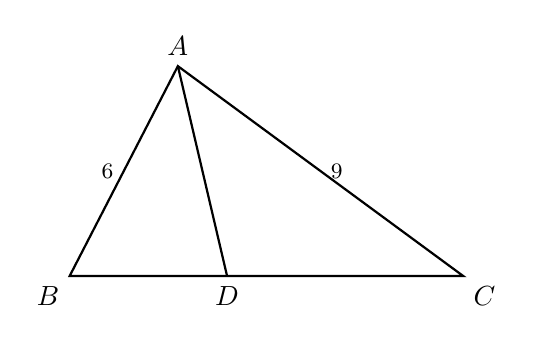
\begin{tikzpicture}[scale=0.5, thick]
  % 用边长 6/9/10 三角形：用余弦律求 A 位置
  % B=(0,0), C=(10,0); cos B = (6^2+10^2-9^2)/(2*6*10)=55/120
  \pgfmathsetmacro{\cosB}{(36+100-81)/(2*6*10)}
  \pgfmathsetmacro{\sinB}{sqrt(1-\cosB*\cosB)}
  \coordinate (B) at (0,0);
  \coordinate (C) at (10,0);
  \coordinate (A) at ({6*\cosB}, {6*\sinB});
  % D 在 BC 上，BD/DC = AB/AC = 6/9 = 2/3 → BD = 4
  \coordinate (D) at (4, 0);

  \draw (A) -- (B) -- (C) -- cycle;
  \draw (A) -- (D);

  \node[above]       at (A) {$A$};
  \node[below left]  at (B) {$B$};
  \node[below right] at (C) {$C$};
  \node[below]       at (D) {$D$};

  \node[left]  at ($(A)!0.5!(B)$) {\footnotesize $6$};
  \node[right] at ($(A)!0.5!(C)$) {\footnotesize $9$};
\end{tikzpicture}
\end{document}
